\documentclass[oneside]{article}
\usepackage{amssymb,amsfonts}
\usepackage{amsthm}
\usepackage{hyperref}
\usepackage{fancyhdr}

\usepackage{graphicx,multicol}
\usepackage{color}

\usepackage[none]{hyphenat} 

\usepackage[left=.75 in,top=.75 in,right=.75 in,bottom=.75 in,nohead]{geometry}

\pagestyle{fancy}
\lfoot{}
\cfoot{\url{http://www.math.ttu.edu/~lhoang/AppliedMath/}}
%\cfoot{\textit{http:/$\!$/www.math.ttu.edu/$\!$\raise-1ex\hbox{{\Large\texttt{\char`\~}}}lhoang/AppliedMath/}}
\rfoot{}
\fancyhead{}
\renewcommand{\headrulewidth}{0pt}


\linespread{1.3}

%%%%%%%%%%%%%%%%%%%%%%%%%%%%%%%%%%%%%%%%%%%%%%%%%%%%%%%%%%%%%%%%%%%%

\newcommand{\talktitle}{Fast Computation of Inverse Transcendentals of Polynomial Expansions through Iterated Means (continued)}

\newcommand{\talkspeaker}{ \textbf{\sc Kevin Long}\\ \textit{Texas Tech University}}

\newcommand{\talkdate}{\textbf{Wednesday, May 1, 2013}}

\newcommand{\timelocation}{\textbf{Room: MATH 109\\  Time: 4:00pm.}}

\newcommand{\talkabstract}{
%
In spectral methods for uncertainty quantification, the output of a system is approximated by a multivariate polynomial of the random inputs. Direct computation of the best $L^2$ multivariate polynomial approximation of a nonlinear function of a multivariate polynomial requires numerical computation of high-dimensional integrals, and can therefore be prohibitively expensive. In 2004, Debusschere {\it et. al.} proposed a method for computing the elementary inverse transcendentals that requires numerical evaluation of one-dimensional integrals, though the integrands become quite complicated.
%
}

\begin{document}

\begin{center}
{\LARGE
Texas Tech University.  Applied Mathematics Seminar.
}
\medskip

\textbf{\Huge {\uppercase{\talktitle}} }

\begin{multicols}{2}
%\begin{center}
{\LARGE
\talkspeaker\\
\talkdate\\
\timelocation
}
%\end{center}

\columnbreak
%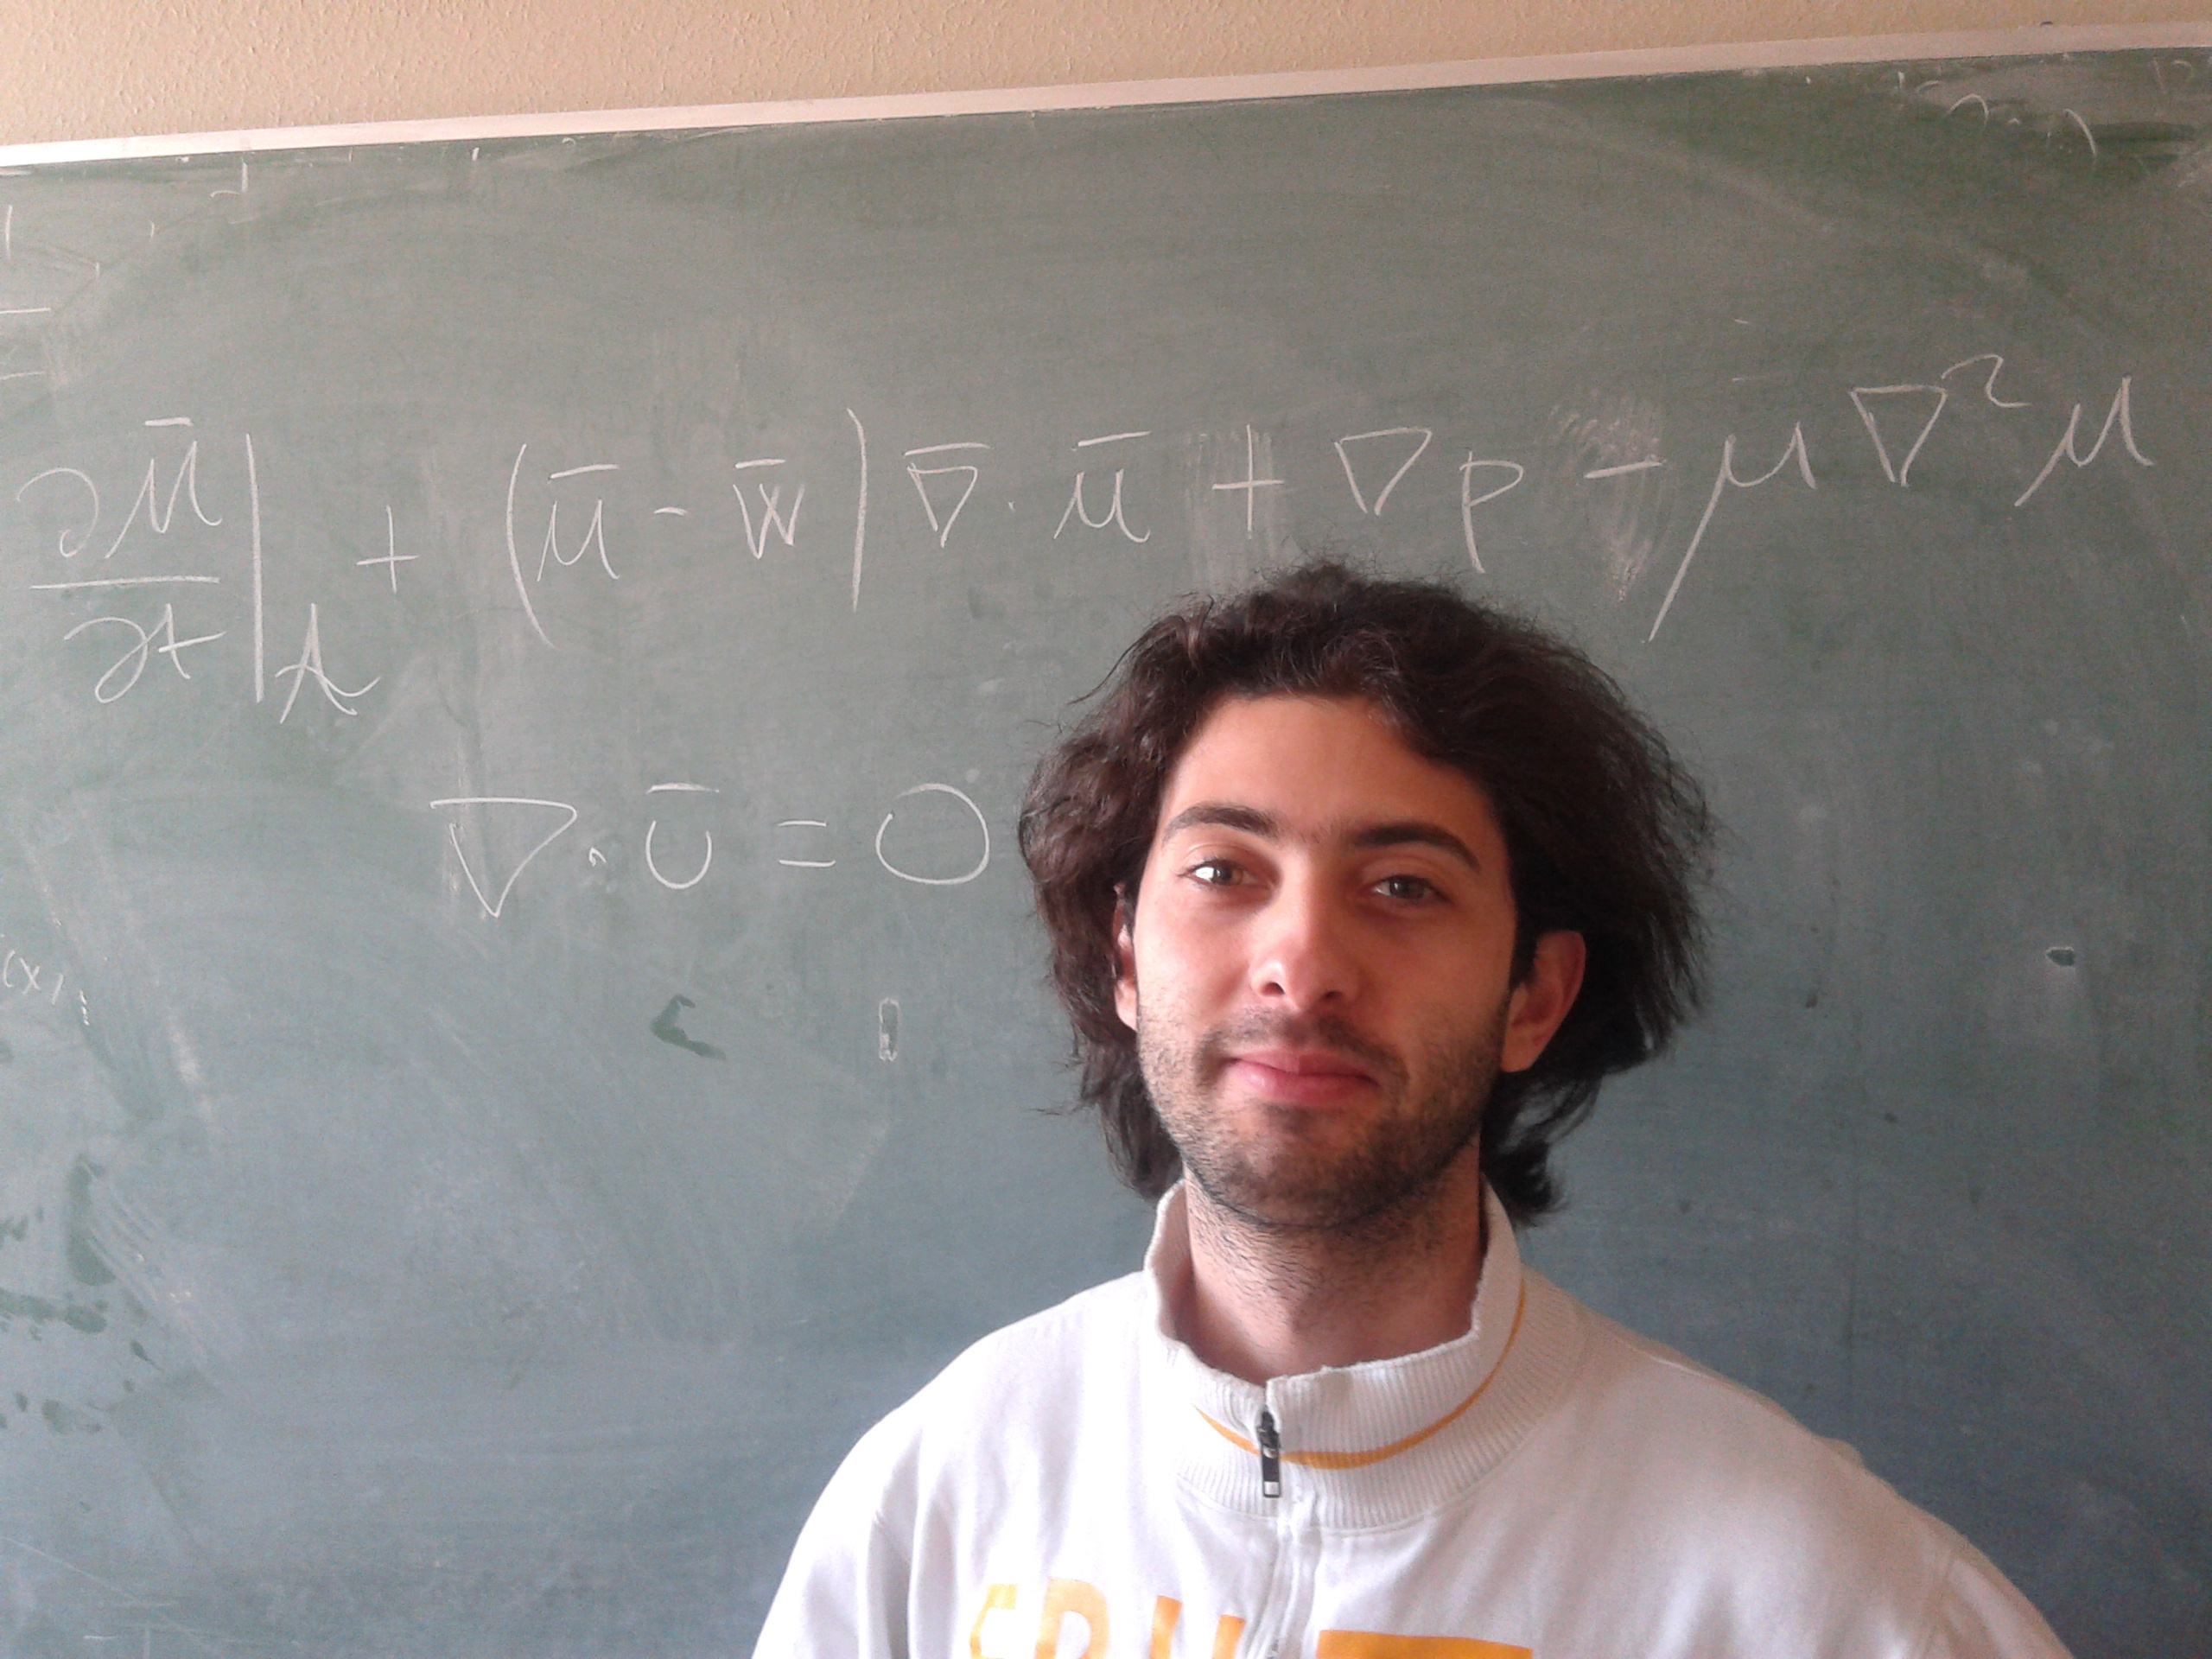
\includegraphics[trim = 25mm 50mm 0mm 20mm, clip, width=2.5in]{Bna.jpg}
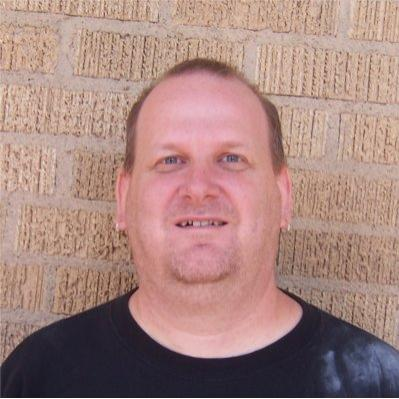
\includegraphics[width=1.8in]{Long.jpg}
\end{multicols}
\end{center}
%\clearpage

\vspace*{-1cm}
\begin{center}
\fbox{\parbox{\linewidth}{
\begin{center}
\begin{minipage}[c]{.96\linewidth}
{
\vspace*{.25cm}
{\LARGE \textbf{ABSTRACT.}}
{\huge \talkabstract}
\vspace*{.25cm}
}
\end{minipage}
\end{center}
}}

\end{center}
\end{document}
